% !TEX root = ./Basilisk-sunSafePoint-20180427.tex

\section{Model Description}

\begin{figure}[t]
	\centerline{
		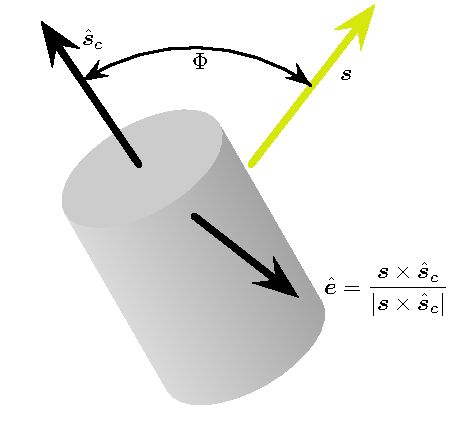
\includegraphics{Figures/sunHeading}
	}
	\caption{Body Vector Illustrations.}
	\label{fig:Fig1}
\end{figure}

\subsection{Module Goal}
This attitude guidance module has the goal of aligning a commanded body-fixed spacecraft vector $\hat{\bm s}_{c}$ with another input vector $\bm s$.  If $\hat{\bm s}_{c}$ is for example the solar panel normal vector, and $\bm s$ is the current sun heading vector, this module will compute the attitude tracking errors to align the solar panels towards the sun, i.e. achieve sun pointing.  Sun pointing is a mode for general recharging the spacecraft, but is also a common guidance scenario with Safe Mode.  

Besides $\bm s$, the second input vector is the inertial body angular velocity vector $\bm\omega_{B/N}$.  The sun pointing frame is assumed to be at rest, thus the attitude rate tracking error is set either equal to the body rates to bring the body to rest, or difference with a specified rotation about the sun heading vector to achieve a final roll about this heading vector.  

As the desired sun pointing orientation is inertial, the inertial reference frame  acceleration $\dot{\bm\omega}_{R/N}$ is set to zero, while the reference rate is either zero or the desired sun-heading roll vector.  

Note that this module does not establish a unique sun-pointing reference frame.  Rather, the pointing condition, align $\hat{\bm s}_{c}$ with $\bm s$ is an under-determined 2 degree of freedom condition.  Thus, the rotation angle about $\bm s$ is left to be arbitrary in this sun pointing module.  For the sun pointing applications this is a very practical result as the power generation does not depend on the orientation about $\bm s$.  



\subsection{Equations}
\subsubsection{Good Sun Direction Vector Case}\label{sec:withSun}
In the following mathematical developments all vectors are assumed to be taken with respect to a body-fixed frame $\cal B$.  The attitude of the body $\cal B$ relative to the reference frame $\cal R$ is written as a principal rotation from $\cal R$ to $\cal B$.  Thus, the associated principal rotation vector $\hat{\bm e}$ is
\begin{equation}
	\label{eq:ssp:1}
	\hat{\bm e} = \frac{\bm s \times \hat{\bm s}_{c}}{|\bm s \times \hat{\bm s}_{c}|}
\end{equation}
Note that the sun direction vector $\bm s$ does not have to be a normalized input vector.  

The principal rotation angle between the two vectors is given through
\begin{equation}
	\label{eq:ssp:2}
	\Phi = \arccos \left( \frac{\bm s  \cdot \hat{\bm s}_{c} }{|\bm s|} \right)
\end{equation}

Next, this rotation from $\cal R$ to $\cal B$ is written as a set of MRPs through
\begin{equation}
	\label{eq:ssp:3}
	\bm\sigma_{B/R} = \tan\left(\frac{\Phi}{4}\right) \hat{\bm e}
\end{equation}
The set $\bm\sigma_{B/R}$ is the attitude error of the output attitude guidance message.  

The module allows for a nominal spin rate about the sun heading axis by specifying the module parameter {\tt sunAxisSpinRate} called $\dot \theta$ in this description.  The nominal spin rate is thus given by
\begin{equation}
	\leftexp{B}{\bm\omega}_{R/N} = \leftexp{B}{\hat{\bm s}} \dot\theta
\end{equation}
Note that this constant nominal spin is only for the case where the sun is visible and the sun-heading vector measurement is available. 

If the spacecraft is to be brought to rest $\bm\omega_{R/N} = \bm 0$, then $\dot\theta$ should be set to zero.  The tracking error angular velocity vector is computed using.
\begin{equation}
	\label{eq:ssp:4}
	\bm\omega_{B/R} = \bm\omega_{B/N} - \bm\omega_{R/N}
\end{equation}

Finally, the attitude guidance message must specify the inertial reference frame  acceleration vector.  This is set to zero as the roll about the sun heading is assumed to have a constant magnitude and inertial heading.
\begin{equation}
	\dot{\bm \omega}_{R/N} = \bm 0
\end{equation}

\subsubsection{No Sun Direction Vector Case}
 If $\Phi$ is less then then module parameter {\tt minUnitMag}, then it is assumed that no good sun heading vector is available and the attitude tracking error $\bm\sigma_{B/R}$ is set to zero.   
 
 Further, if the sun is not visible, the module allows for a non-zero body rate to be prescribed.  This allows the spacecraft to engage in a constant rate tumble specified through the module configuration vector {\tt omega\_RN\_B}.  In this case the tracking error rate is evaluate through
 \begin{equation}
 	\label{eq:ssp:6}
	\bm\omega_{B/R} = \bm\omega_{B/N} - \bm\omega_{R/N}
 \end{equation}
 and the output message reference rate is set equal to the prescribed $\bm\omega_{R/N}$ while the reference acceleration vector $\dot{\bm \omega}_{R/N}$ is set to zero.

 
 \subsubsection{Collinear Commanded and Sun Heading Vectors}
First consider the case where $\bm s \approx \hat{\bm s}_{c}$.  In this case the cross product in Eq.~\eqref{eq:ssp:1} is not well defined.  Let $\epsilon$ be a pre-determined small angle.  Then, if $\Phi < \epsilon$ the attitude tracking error is set to 
$$
	\bm\sigma_{B/R} = \bm 0
$$
 
 
However, if $\bm s \approx -\hat{\bm s}_{c}$, then an eigen-axis $\hat{\bm e}$ that is orthogonal to $\hat{\bm s}_{c}$ must be determined.  Let the body frame be defined through \frameDefinition{B}.  The eigen-axis is determined first by taking a cross product with $\hat{\bm b}_{1}$:
 \begin{equation}
	\label{eq:ssp:7}
	\hat{\bm e}_{180} = \frac{ \hat{\bm s}_{c} \times \hat{\bm b}_{1}}{| \hat{\bm s}_{c} \times \hat{\bm b}_{1}|}
\end{equation}
If $\hat{\bm s}_{c} \approx \hat{\bm b}_{1}$, then this $\hat{\bm e}$ vector will have a small norm.  In this ill-determined case, the $\hat{\bm e}$ vector is determined using
 \begin{equation}
	\label{eq:ssp:8}
	\hat{\bm e}_{180} = \frac{ \hat{\bm s}_{c} \times \hat{\bm b}_{2}}{| \hat{\bm s}_{c} \times \hat{\bm b}_{2}|}
\end{equation}
As $ \hat{\bm s}_{c}$ cannot both be aligned with $\hat{\bm b}_{1}$ and $\hat{\bm b}_{2}$, this algorithm determines a unique eigen axis $\hat{\bm e}_{180}$ for the case that the principal rotation angle is close to 180 degrees, or $\pi - \Phi < \epsilon$.  This special case eigen axis is only computed once in the module reset routine.

In this scenario the angular velocity tracking error is evaluated using the same method as outlined in section~\ref{sec:withSun}.
 
 